\section{Analysis}

I want to introduce our development process using a flowchart combined with illustration.

\begin{figure}[htb]
    \centering
    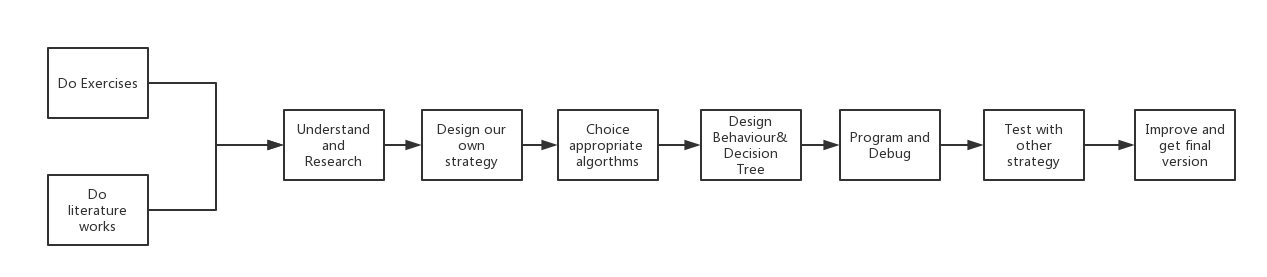
\includegraphics[width=1\textwidth]{images/flow_chart.png}
    \caption{Flow Chart of Development Process}
    \label{figure:flow_chart}
\end{figure}

The first thing we considered about our strategy is the search algorithm, taking that all
possible point positions are not that many into consideration, it will not require much memory
space than using DFS. Also using BFS pathfinding strategy is much quicker. Also, we did not use
any informed search algorithms so that we can diminish computation time and react quicker, since
all informed algorithms will need more time to calculate the best combination of actions. 

So the main goal of implementing BFS algorithm is to reduce the computation time of search based
on acceptable non-optimal algorithms, and arrange actions as fast as possible instead of using search
algorithms to calculate combination of actions to find optimal moves. By controlling the choices
points of each unit we created in uRTS, we can meet the given time constraints and results in a
quicker reaction and a more simplified AI system. Assuming that we are creating a quickly reactive
system in uRTS game. In this case we will allow scripts to expose only a few carefully chosen choice
points, if at all, resulting in fast searches that may sometimes miss optimal moves, but generally produce
acceptable action sequences quickly\cite{barriga2018game}. So, our bot is based on decision tree
which can minimize the effect of RTS constraints so that the bot can gener-ate sequence of actions
very quickly. Meanwhile, to maximize our advantage of ‘quickly generated action sequence’, we guarantee
that every decision made will lead to a certain action. 

We compared all hard-coded strategies, including WorkerRush, LightRush, Heavy-Rush and RangedRush, and
then tested them against each other, we found that WorkerRush is quickest rush strategy and it remain
a high wining rate among all strategies, so we decided to improve it by using our own Tree. When there
is no more branch of tree, algorithm will turn to another state or branch to continue executing decisions.
Decisions of each node are made by value of parameters in our program, decision tree is quite fast and
easy to implement in deciding which action an unit should do during the configuration of our agent. 

The Tree is shown as Figure \ref{figure:tree_of_group_g}.

\begin{figure}[htb]
    \centering
    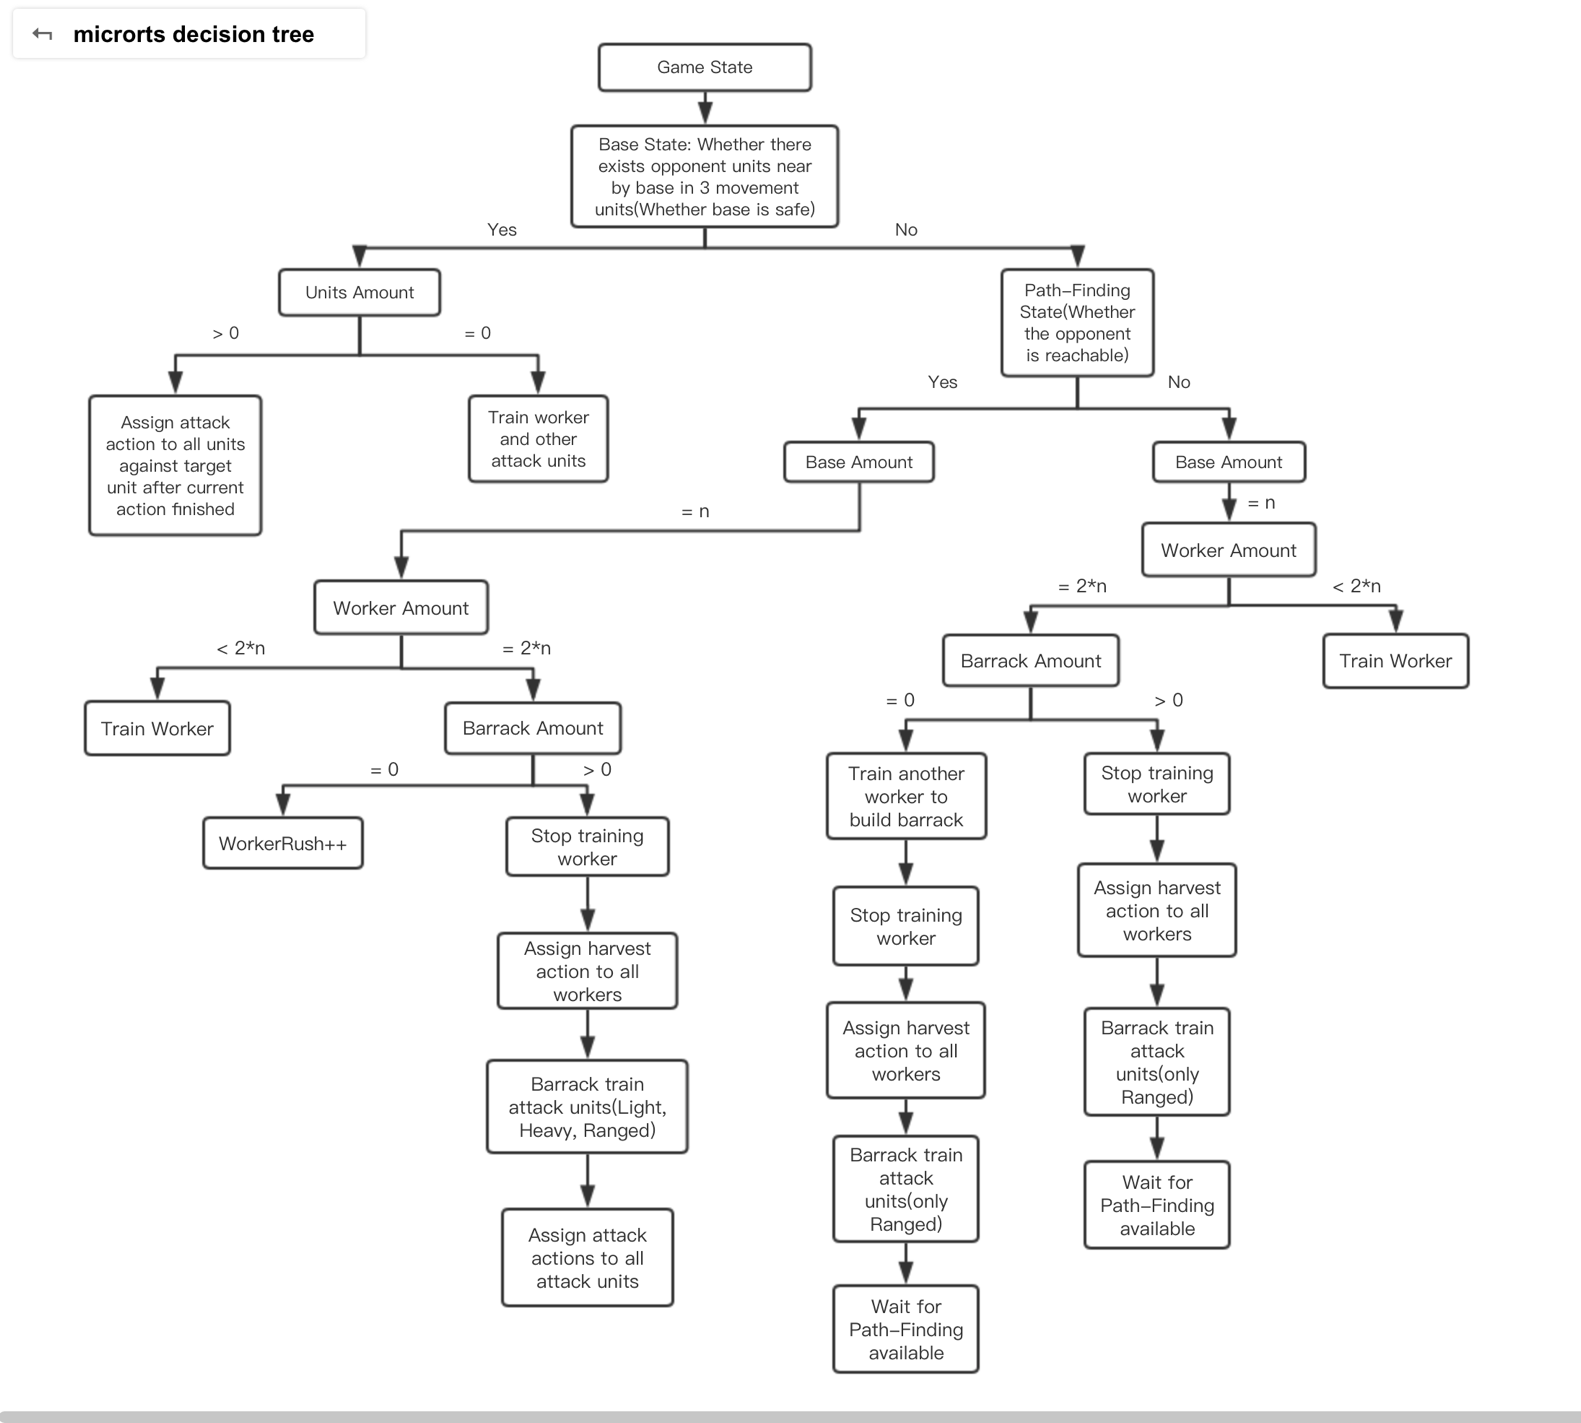
\includegraphics[width=1\textwidth]{images/tree_of_group_g.png}
    \caption{Decision Tree of Group G}
    \label{figure:tree_of_group_g}
\end{figure}

As you can see from the Figure \ref{figure:tree_of_group_g}, our Tree is more like a Decision Tree combined with
a Behaviour Tree, some nodes represent decision conditions and others represent actions. The required
returned value depends on what kind of action the nodes take and the unit condition. 

At the beginning node (root) of the tree, we will consider the security of our base, if there are any enemy
units around it within 3 movements, if the base is not safe, the system will assign units to attack enemies
until they all dead. Otherwise, when the base is safe (There are more than 3 movements between our base),
the system will do options depends on different types of map. 

So, when the system confirm base is in a safe condition, the system will decide which map we are using now
according to the Barrack Amount and if opponents are reach-able (Opponents are not reachable in the map with
resources blocked in the middle). There are four different types of maps, so we decide different strategies
to reply to them. 

The first two types of maps are very similar but has different size and resource, so we directly train worker
units until the number fits our condition, then control all workers to attack.

\begin{figure}[htb]
    \centering
    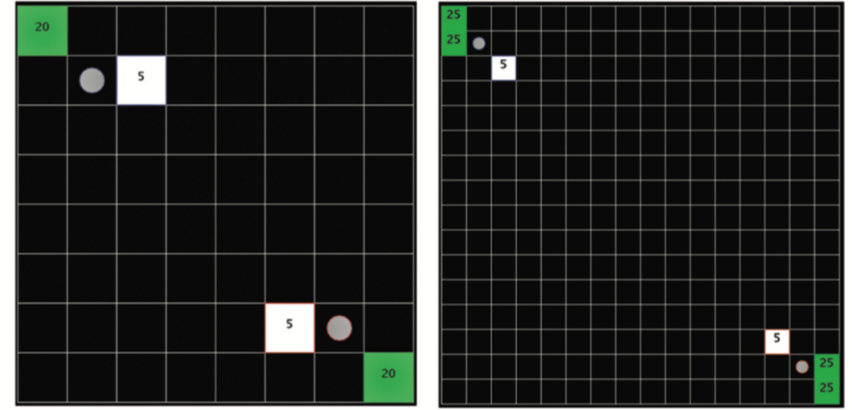
\includegraphics[width=0.6\textwidth]{images/first_two_maps.png}
    \caption{First Two Maps}
    \label{figure:first_two_maps}
\end{figure}

When it comes with map with Barracks, we will assign harvest action to all workers and train all kinds of
attack units. Then we assign attack actions to units.

\begin{figure}[htb]
    \centering
    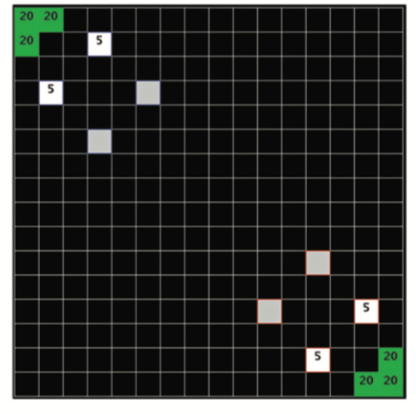
\includegraphics[width=0.4\textwidth]{images/map_with_initial_barracks.png}
    \caption{Map with Initial Barracks}
    \label{figure:map_with_initial_barracks}
\end{figure}

Last is the type of map that opponents are not reachable at the beginning, at this situation we will execute
a different strategy: First we train workers and let them build Barracks, after that let workers harvest to get
resources. Then build Ranged Attack Units to attack. In this way, our system can do it best to train Ranged Attack
Units, which has huge advantage in this map.

At last, we run some tests between our bot and built-in strategies bot on 4 maps:
\begin{enumerate}
    \item baseWorkers16x16
    \item baseWorkers24x24H
    \item TwoBasesBarracks16x16
    \item NoWhereToRun9x8
\end{enumerate}
In each map, we switched the position of twobots to run the test. The results are shown in Table \ref{table:test_result}.

\begin{table}[h]
    \centering
    \caption{Test results of our bot vs other bots. '1' represents our bot wins and '0' represents our bots lose}
    \label{table:test_result}
    \begin{tabular}{|c|c|c|c|c|c|c|c|c|}
        \toprule
        Map & \multicolumn{2}{|c|}{map1} & \multicolumn{2}{|c|}{map2}
            & \multicolumn{2}{|c|}{map3} & \multicolumn{2}{|c|}{map4} \\
        \midrule
        Position & ai1 & ai2 & ai1 & ai2 & ai1 & ai2 & ai1 & ai2 \\
        \midrule
        WR++     &  0  &  1  &  0  &  0  &  1  &  1  &  1  &  1  \\
        HR       &  1  &  1  &  1  &  1  &  1  &  1  &  1  &  1  \\
        LR       &  1  &  1  &  1  &  1  &  1  &  1  &  1  &  1  \\
        RR       &  1  &  1  &  1  &  1  &  1  &  1  &  1  &  1  \\
        SER      &  1  &  1  &  1  &  1  &  1  &  1  &  1  &  1  \\
        \bottomrule
    \end{tabular}
\end{table}

From the charts we noticed that our tactical bot performs as good as expectation on most map, the only two battles
that we lose is on the map with single base and no barracks against our ‘parents’ strategy ‘WorkerRushPlusPlus’.
Because in our behaviour tree, when the game state is path-finding available and no barracks at initial state,
our bot behaves as similar as ‘WorkerRushPlusPlus’. During the test two bots were locked in the battle but our
bot finally lose the game, only defeat enemy once when at the position of ai2 on ‘baseWorkers16x16’. We will
work on this and make progress and improvement in the future.
